% !TeX spellcheck = fr_FR
\chapter{Chapitre 1 : Données et formats}

% \begin{center}
% 	\textit{Chaque chapitre doit commencer sur une nouvelle page.}\\*[35pt]
% \end{center}

Dans ce chapitre nous allons aborder les différents format de données qui seront
cités dans la suite de ce document.

\section{Données lidar}

\gls{lidar} ou en français 
détection et estimation de la distance par la lumière est une technique de mesure de distance où la lumière réalise un 
aller-retour entre sa source et un objet. On chronomètre le temps entre le moment 
où une pulsation de lumière est émise par un laser et son retour vers un capteur.
En connaissant la vitesse de propagation de la lumière dans l’environnement où elle
évolue, il est possible de déterminer la distance qui sépare l’objet 
du capteur. Plus précisément, il s’agit de la distance séparant le dispositif de
mesure et un point de l’objet frappé par la lumière émise. 
Cette opération effectuée à de multiples reprises en changeant par petit pas 
l’angle du laser, créer des points supplémentaires qui une fois réunis,
constituent un nuage de points profilant l'environnement autour de l'instrument.
Si l'instrument de mesure est placé sur un avion et que la source de lumière est
dirigée vers le bas, il est ainsi possible de capturer, sous forme d'un nuage de
points, une région du globe. Ce cas nécessite tout de fois de connaître la position
du \gls{gps} de l'avion au moment de la capture d'un point afin de mettre en relation
tous les points à la fin de la mesure.
Il existe différentes versions de la spécification et ce document va se concentrer sur la version un point deux.



Le format de stockage des nuages de points de données \gls{lidar}, est un format
binaire dont les spécifications sont définies par l'\gls{asprs}.
Le format \gls{las} est composé de trois sections, respectivement:
L'en-tête de fichier, les enregistrement à longueur variable et les données lier aux points récoltés.

\begin{table}[!h]
    \centering
    \begin{tabular}{ |c|c| }
        \hline
        En-tête \\
        \hline
        Enregistrements à longueur variable \\
        \hline
        Données des points \\
        \hline
    \end{tabular}
    \caption[Sections composant un fichier au format LAS]{
            Sections composant un fichier au format LAS, 
            Source: adapté de LAS Specification Version 1.2 (2008, p. 2)
    }
    \label{tab:las_sections}
\end{table}
\newpage
Dans toutes les sections, on défini les types de données dans le tableau \ref{tab:data_type}
\begin{table}[!htb]
    \centering
    \begin{tabular}{|l|c|}
    \hline
    \textbf{Type de donnée}           & \textbf{Nombre d'octets} \\ \hline
    char           & 1               \\ \hline
    unsigned  char & 1               \\ \hline
    short          & 2               \\ \hline
    unsigned short & 2               \\ \hline
    long           & 4               \\ \hline
    unsigned long  & 4               \\ \hline
    double \tablefootnote{selon le standard IEEE 754} & 8     \\ \hline
    \end{tabular}
    
    \caption[Type de données de la définition du format LAS]{
        Type de données de la définition du format LAS,
        Source: adapté de LAS Specification Version 1.2 (2008, p. 2-3)
    }
    
    % tiré de Tartempion 2010, p. 42 / tiré de ce-site.ch, ref. URL02 / réalisé par Nom Prénom.}
    \label{tab:data_type}
\end{table}

\subsection{En-tête publique}

L'en-tête publique comporte les métadonnées du fichier.
Il est composé de tous les champs du tableau \ref {tab:las_header} présent dans l'annexe 1.
Tous les champs inutilisés doivent être remplis par des bits nuls et les champs sont au format little endian.
La signature de fichier doit obligatoirement contenir les quatre caractères “LASF” et est requise par la spécification.
Un programme lisant le fichier doit vérifier cette signature pour déterminer qu’il s’agisse bien d’un fichier \gls{las}.

Parmi les champs, les facteurs $ X, Y $ et $ Z $ scale sont utilisés avec les valeurs $ X, Y$ et $Z$ offset pour obtenir des coordonnées cartésiennes des axes.
Ces valeurs sont globales au fichier. Voici la formule pour chacune.  

\begin{equation}
    X_{coordinates} = (X_{enregistrement} * X_{scale}) + X_{offset}
\end{equation}


\section{Format Stéréoligraphique}
\section{Format VTK}

% \begin{figure}[tbph!]
% 	\centering
% 	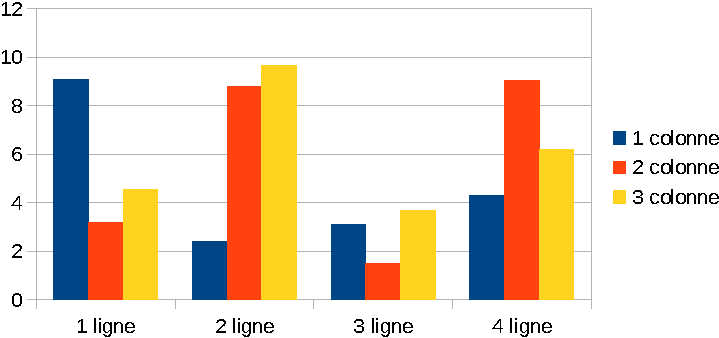
\includegraphics[width=0.7\linewidth]{chart}
% 	\caption[Diagramme machin]{Diagramme machin. Source : tiré de Tartempion 2010, p. 42 / tiré de ce-site.ch, ref. URL01 / réalisé par Nom Prénom.}
% 	\label{fig:chart1}
% \end{figure}
% 
% 
% \begin{table}[tbph!]
% 	\centering{
% 		\begin{tabular}{ |l|c|c|c| }
% 			\hline
% 			& \textbf{Condition 1} & \textbf{Condition 2} & \textbf{Condition 3} \\
% 			\hline
% 			\textbf{Test 1} & X & O & X \\
% 			\hline
% 			\textbf{Test 2} & O & X & X \\
% 			\hline
% 			\textbf{Test 3} & O & X & O \\
% 			\hline 
% 		\end{tabular}
% 		\caption[Lot de données n°1]{Lot de données n°1. Source: tiré de Tartempion 2010, p. 42 / tiré de ce-site.ch, ref. URL02 / réalisé par Nom Prénom.}
% 		\label{tab:tableau1}
% 	}
% \end{table}
% 
% 
% \begin{figure}[tbph!]
% 	\centering
% 	
\includegraphics[width=0.7\linewidth]{diagram}
% 	\caption[Schéma bidule.]{Schéma bidule. Source : tiré de Tartempion 2010, p. 42 / tiré de ce-site.ch, ref. URL03 / réalisé par Nom Prénom.}
% 	\label{fig:diagram}
% \end{figure}
% 
% 
% \section{Titre de niveau 2}
% 
% 
% \begin{figure}[tbph!]
% 	\centering
% 	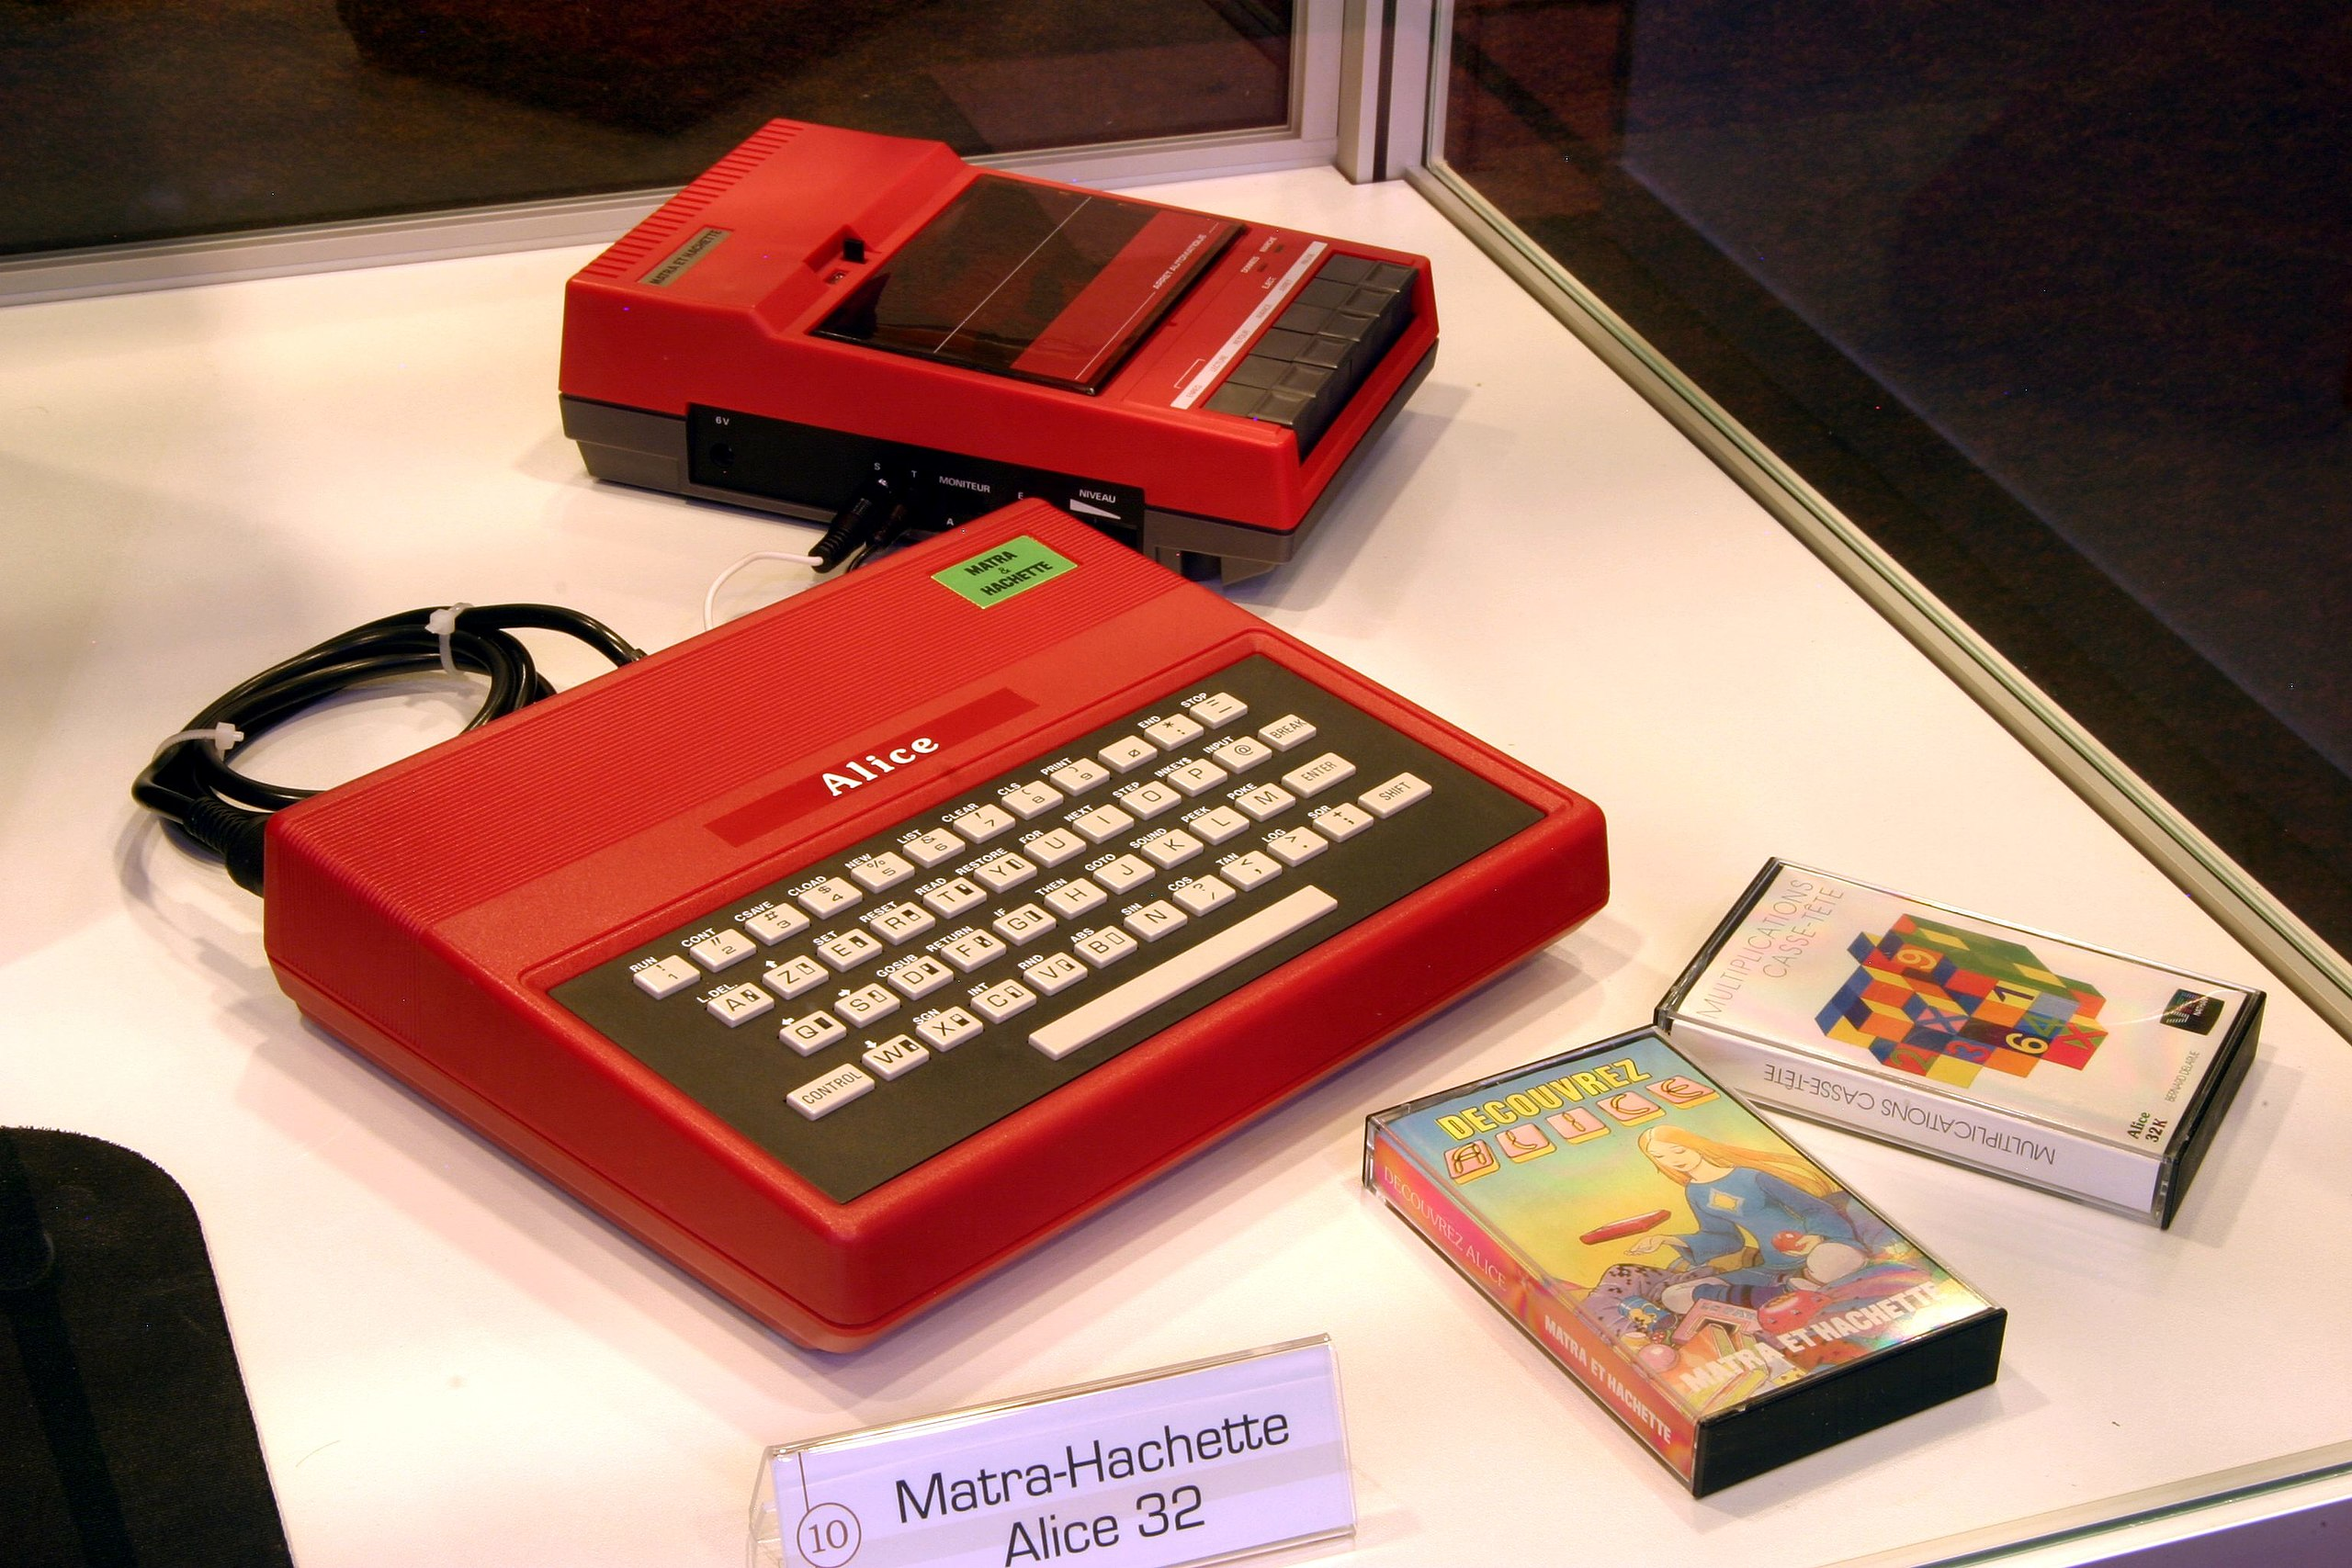
\includegraphics[width=0.7\linewidth]{ordi}
% 	\caption[Alice, Micro-ordinateur MATRA.]{Alice, Micro-ordinateur MATRA. Source : tiré de Tartempion 2010, p. 42 / tiré de ce-site.ch, ref. URL03 / réalisé par Nom Prénom.}
% 	\label{fig:image}
% \end{figure}
% 
% 
% \subsection{Titre de niveau 3}
% 
% 
% \begin{table}[tbph!]
% 	\centering{
% 		\begin{tabular}{ |l|c|c|c| }
% 			\hline
% 			& \textbf{Condition 1} & \textbf{Condition 2} & \textbf{Condition 3} \\
% 			\hline
% 			\textbf{Test 1} & X & O & X \\
% 			\hline
% 			\textbf{Test 2} & O & X & X \\
% 			\hline
% 			\textbf{Test 3} & O & X & O \\
% 			\hline 
% 		\end{tabular}
% 		\caption[Lot de données n°2.]{Lot de données n°2. Source: tiré de Tartempion 2010, p. 42 / tiré de ce-site.ch, ref. URL05 / réalisé par Nom Prénom.}
% 		\label{tab:tableau2}
% 	}
% \end{table}
